\documentclass[12pt]{report}
\usepackage{hyperref}
\hypersetup{
	colorlinks=true,
	linkcolor=blue,
	filecolor=magenta,
	urlcolor=cyan,
	pdftitle={Overleaf Example},
	pdfpagemode=FullScreen,
}
\usepackage{csquotes}
\usepackage{graphicx}

\title{AI code generation report}
\author{Roblox prime numbers:\\\small{Oleh Basystyi}\\\small{Anna Stasyshyn}
\\\small{Artur Rudish}\\\small{Anton Valihurskyi}\\\small{Maksym Zhuk}}
\date{April 2024}
\begin{document}
	\maketitle
	\renewcommand{\thesection}{\arabic{section}}
	\section{Introduction}
	\qquad In this little research, our team researched AI's capability to solve CodeWars tasks of different difficulty (in particular, 7 to 4 kyu) and different CodeWars categories:
	\begin{itemize}
		\itemsep0em
		\item Algorithms
		\item Strings
		\item Arrays
		\item Mathematics
		\item Linear Algebra
		\item Dynamic Programming
		\item Data Structures
	\end{itemize}
	\qquad As for AIs, we used \textit{GPT-3.5, GPT-4, Claude} and \textit{Gemini} to create an aggregated conclusion about AI code generation. In addition, we researched two different approaches to writing prompts to solve problems: templated and manual (must be used in different cases).

	\pagebreak
	\section{Setup of experiments and general conclusions}
	\qquad To carefully carry out experiments, we set up a \href{https://docs.google.com/spreadsheets/d/1qXPyAJsOOpmtxIoGqObwG5mTaLU3IWO0SQRGbjZPhEc/edit#gid=0}{Google Sheets table} to log data about AIs' problem-solving performance by following metrics: \textit{Prompts used to solve problem, Number of times when AI returned code that didn't pass all the test cases, Number of times when AI returned code that had runtime errors, and number of consecutive prompts when AI got stuck on the same problem} In total, we analyzed 18 problems and gained the following data:

	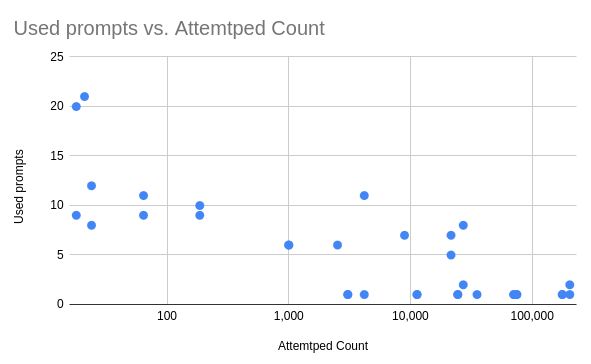
\includegraphics[width=\textwidth]{used_prompts_attempted_relation.png}

	It shows the relation between the number of people who attempted to solve a particular problem and the number of prompts that we used to make AI solve it. As shown on the chart, the general rule is that tasks with a lower attempt count were more difficult to solve by AI. Our assumption is that this relation occurs because AI has less variants of training data (\textit{actual solution on CodeWars, Reddit and StackOverflow threads}). Moreover, we can see a breakpoint at approximately 1000 attempts, where we had to increase the number of prompts to solve the problem. As a result, we used different techniques to get the problem solution from AI. Interestingly, even \textbf{kyu difficulty} doesn't define AI's performance as much as \textbf{attempted count} do (see the \href{https://docs.google.com/spreadsheets/d/1qXPyAJsOOpmtxIoGqObwG5mTaLU3IWO0SQRGbjZPhEc/edit#gid=0}{table} from 14th to 20th row).

	\subsection{Generating solutions to problems with a big number of attempts}

		We concluded that a problem that has an \textbf{attempt count} of more than 4,000 requires one or two prompts similar to the ones below:

		\begin{itemize}
			\itemsep0em
			\item Solve this problem using python: \textbf{[provided problem description]} and use function prototype \textbf{[function prototype]}
		   \item Your code should satisfy these test cases \textbf{[failed test cases]}
		   \item Please optimize your solution
		\end{itemize}

		However, there are several exceptions from this rule. Even if a 2-3 kyu problem has over 4,000 attempts, AI can't solve this problem due to the complexity of its descriptions and many definitions that AI fails to understand properly. Secondly, even if problems of 7-8 kyu have a small attempt count, AI can solve it (see the \href{https://docs.google.com/spreadsheets/d/1qXPyAJsOOpmtxIoGqObwG5mTaLU3IWO0SQRGbjZPhEc/edit#gid=0}{table} from 14th to 20th row).

	   What we have also discovered is that AI can sometimes get stuck on a simple problem, but after creating a new chat, it manages to solve in one or two prompts worded similarly to the ones listed above (see the \href{https://docs.google.com/spreadsheets/d/1qXPyAJsOOpmtxIoGqObwG5mTaLU3IWO0SQRGbjZPhEc/edit#gid=0}{table} second row).

	\subsection{Generating solutions to problems with a small number of attempts}
		\qquad In our tests, we discovered that if a problem has less than 500 \textit{solution attempts}, AI cannot solve it using the three types of prompts listed above. AI searches for a solution in the right directioin but always misses some details. In that case, these mistakes must be fixed maually. For example, let us take a look at what we used to direct the AIs to help them solve the problems:

		\begin{itemize}
			\item\href{https://www.codewars.com/kata/57e32bb7ec7d241045000661}{Diophantine Equation Solver} is a 6 kyu problem but has only \textit{64} solution attempts, so both Claude and ChatGPT-3.5 couldn't solve it just from problem's description. The AIs generated a valid basic structure of the solution, but we corrected it with proper for-loop boundaries and told them to select solutions with the maximum possible $z$. After that, they forgot to count all the solutions, so we had to remind to add a counter as well. We used the following prompts: \textit{"In fact, using number theory, we can prove that the limit for y is math.floor(math.sqrt((z*z*z)/3))"}, \textit{"But now you must introduce a counter for all the solutions."} - there were more of them, but these are the main ones.
			\item\href{https://www.codewars.com/kata/5901aee0af945e3a35000068/train/python}{3 Matrices: Rearrange the matrix}, with a difficulty of 5 kyu and 24 total solutions, was solved. At first, both models provided non-working code that couldn't be fixed. However, after creating a new chat and providing libraries that should have been used, GPT-3.5 solved it on the \textit{"first"} try, but Gemini still couldn't solve it.

		\end{itemize}


		To sum everything up, AIs nowadays are incapable of deep reasoning when there are not many similar examples. After being prompted to solve one problem in their code, another one occurs.

	\subsection{Unsolved problems}
		\qquad As mentioned before, LLMs showed poor performance in solving unpopular problems. If there are not many similar problem solutions on the internet, troubles arise: at first, models could not find an appropriate approach for the problem, which led to erroneous code or incorrect solutions. After a few consecutive prompts providing models with failed test cases, LLMs tweaked the code a little bit but made no difference. Then, we tried providing models with hints on the correct approach, based on existing valid solutions, they remade the code, and a small part of the tests passed but they still were not able to make their code pass all the tests. In such cases, there is no use in AI as we enter a cycle of reccurent errors. We could not manage to solve all the planned problems. Unsolved tasks can be seen in the \href{https://docs.google.com/spreadsheets/d/1qXPyAJsOOpmtxIoGqObwG5mTaLU3IWO0SQRGbjZPhEc/edit#gid=0}{table} (highlighted with gray).

	\section{Recommendations for AI code generation}
		\qquad Using collected data, we created the following guidelines (algorithm) for AI code generation:

		\begin{enumerate}
			\item Determine whether your problem is popular or very specific.
			\item In case it is widespread, you can simply use the problem's description in a prompt, and, most likely, you will get the right solution.
			\item If you determined that your problem is not narrowly focused, you should:
			\begin{enumerate}
				\item Think of a straight-forward solution and then feed the problem's description to the AI.
				\item Check if the AI solution is going in the right direction and determine the main AI's mistakes.
				\item Remind the AI of those mistakes one-by-one in your prompts.
				\item Repeat steps (b) and (c) until the AI returns the right solution.
			\end{enumerate}
		\end{enumerate}

		Additionally, do not try to feed the whole problem if it has a lot of abstract definitions, classes and functions that are narrowly focused on your task. Try to split the problem into smaller parts, preferably into functions and solve them accordingly.

	\section{Conclusions}
		\qquad In this research we discovered that AI nowadays is capable of efficient problem-solving if there are many solutions to similar problems on the internet or they are considerably easy. We cannot feed a problem with vast definitions and examples and hope that AI can proccess it. Code generation can only be used to lessen the repetetive manual work of solving trivial problems or searching for directions in solving hard problems as discussed in Section 2.2.


\end{document}
